\documentclass[1p]{elsarticle_modified}
%\bibliographystyle{elsarticle-num}

%\usepackage[colorlinks]{hyperref}
%\usepackage{abbrmath_seonhwa} %\Abb, \Ascr, \Acal ,\Abf, \Afrak
\usepackage{amsfonts}
\usepackage{amssymb}
\usepackage{amsmath}
\usepackage{amsthm}
\usepackage{scalefnt}
\usepackage{amsbsy}
\usepackage{kotex}
\usepackage{caption}
\usepackage{subfig}
\usepackage{color}
\usepackage{graphicx}
\usepackage{xcolor} %% white, black, red, green, blue, cyan, magenta, yellow
\usepackage{float}
\usepackage{setspace}
\usepackage{hyperref}

\usepackage{tikz}
\usetikzlibrary{arrows}

\usepackage{multirow}
\usepackage{array} % fixed length table
\usepackage{hhline}

%%%%%%%%%%%%%%%%%%%%%
\makeatletter
\renewcommand*\env@matrix[1][\arraystretch]{%
	\edef\arraystretch{#1}%
	\hskip -\arraycolsep
	\let\@ifnextchar\new@ifnextchar
	\array{*\c@MaxMatrixCols c}}
\makeatother %https://tex.stackexchange.com/questions/14071/how-can-i-increase-the-line-spacing-in-a-matrix
%%%%%%%%%%%%%%%

\usepackage[normalem]{ulem}

\newcommand{\msout}[1]{\ifmmode\text{\sout{\ensuremath{#1}}}\else\sout{#1}\fi}
%SOURCE: \msout is \stkout macro in https://tex.stackexchange.com/questions/20609/strikeout-in-math-mode

\newcommand{\cancel}[1]{
	\ifmmode
	{\color{red}\msout{#1}}
	\else
	{\color{red}\sout{#1}}
	\fi
}

\newcommand{\add}[1]{
	{\color{blue}\uwave{#1}}
}

\newcommand{\replace}[2]{
	\ifmmode
	{\color{red}\msout{#1}}{\color{blue}\uwave{#2}}
	\else
	{\color{red}\sout{#1}}{\color{blue}\uwave{#2}}
	\fi
}

\newcommand{\Sol}{\mathcal{S}} %segment
\newcommand{\D}{D} %diagram
\newcommand{\A}{\mathcal{A}} %arc


%%%%%%%%%%%%%%%%%%%%%%%%%%%%%5 test

\def\sl{\operatorname{\textup{SL}}(2,\Cbb)}
\def\psl{\operatorname{\textup{PSL}}(2,\Cbb)}
\def\quan{\mkern 1mu \triangleright \mkern 1mu}

\theoremstyle{definition}
\newtheorem{thm}{Theorem}[section]
\newtheorem{prop}[thm]{Proposition}
\newtheorem{lem}[thm]{Lemma}
\newtheorem{ques}[thm]{Question}
\newtheorem{cor}[thm]{Corollary}
\newtheorem{defn}[thm]{Definition}
\newtheorem{exam}[thm]{Example}
\newtheorem{rmk}[thm]{Remark}
\newtheorem{alg}[thm]{Algorithm}

\newcommand{\I}{\sqrt{-1}}
\begin{document}

%\begin{frontmatter}
%
%\title{Boundary parabolic representations of knots up to 8 crossings}
%
%%% Group authors per affiliation:
%\author{Yunhi Cho} 
%\address{Department of Mathematics, University of Seoul, Seoul, Korea}
%\ead{yhcho@uos.ac.kr}
%
%
%\author{Seonhwa Kim} %\fnref{s_kim}}
%\address{Center for Geometry and Physics, Institute for Basic Science, Pohang, 37673, Korea}
%\ead{ryeona17@ibs.re.kr}
%
%\author{Hyuk Kim}
%\address{Department of Mathematical Sciences, Seoul National University, Seoul 08826, Korea}
%\ead{hyukkim@snu.ac.kr}
%
%\author{Seokbeom Yoon}
%\address{Department of Mathematical Sciences, Seoul National University, Seoul, 08826,  Korea}
%\ead{sbyoon15@snu.ac.kr}
%
%\begin{abstract}
%We find all boundary parabolic representation of knots up to 8 crossings.
%
%\end{abstract}
%\begin{keyword}
%    \MSC[2010] 57M25 
%\end{keyword}
%
%\end{frontmatter}

%\linenumbers
%\tableofcontents
%
\newcommand\colored[1]{\textcolor{white}{\rule[-0.35ex]{0.8em}{1.4ex}}\kern-0.8em\color{red} #1}%
%\newcommand\colored[1]{\textcolor{white}{ #1}\kern-2.17ex	\textcolor{white}{ #1}\kern-1.81ex	\textcolor{white}{ #1}\kern-2.15ex\color{red}#1	}

{\Large $\underline{12n_{0406}~(K12n_{0406})}$}

\setlength{\tabcolsep}{10pt}
\renewcommand{\arraystretch}{1.6}
\vspace{1cm}\begin{tabular}{m{100pt}>{\centering\arraybackslash}m{274pt}}
\multirow{5}{120pt}{
	\centering
	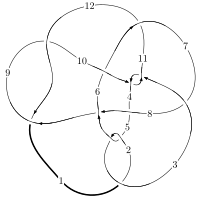
\includegraphics[width=112pt]{../../../GIT/diagram.site/Diagrams/png/2495_12n_0406.png}\\
\ \ \ A knot diagram\footnotemark}&
\allowdisplaybreaks
\textbf{Linearized knot diagam} \\
\cline{2-2}
 &
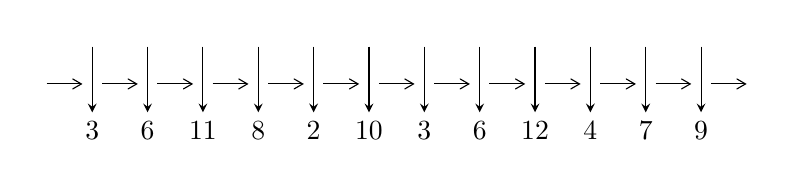
\begin{tikzpicture}[x=20pt, y=17pt]
	% nodes
	\node (C0) at (0, 0) {};
	\node (C1) at (1, 0) {};
	\node (C1U) at (1, +1) {};
	\node (C1D) at (1, -1) {3};

	\node (C2) at (2, 0) {};
	\node (C2U) at (2, +1) {};
	\node (C2D) at (2, -1) {6};

	\node (C3) at (3, 0) {};
	\node (C3U) at (3, +1) {};
	\node (C3D) at (3, -1) {11};

	\node (C4) at (4, 0) {};
	\node (C4U) at (4, +1) {};
	\node (C4D) at (4, -1) {8};

	\node (C5) at (5, 0) {};
	\node (C5U) at (5, +1) {};
	\node (C5D) at (5, -1) {2};

	\node (C6) at (6, 0) {};
	\node (C6U) at (6, +1) {};
	\node (C6D) at (6, -1) {10};

	\node (C7) at (7, 0) {};
	\node (C7U) at (7, +1) {};
	\node (C7D) at (7, -1) {3};

	\node (C8) at (8, 0) {};
	\node (C8U) at (8, +1) {};
	\node (C8D) at (8, -1) {6};

	\node (C9) at (9, 0) {};
	\node (C9U) at (9, +1) {};
	\node (C9D) at (9, -1) {12};

	\node (C10) at (10, 0) {};
	\node (C10U) at (10, +1) {};
	\node (C10D) at (10, -1) {4};

	\node (C11) at (11, 0) {};
	\node (C11U) at (11, +1) {};
	\node (C11D) at (11, -1) {7};

	\node (C12) at (12, 0) {};
	\node (C12U) at (12, +1) {};
	\node (C12D) at (12, -1) {9};
	\node (C13) at (13, 0) {};

	% arrows
	\draw[->,>={angle 60}]
	(C0) edge (C1) (C1) edge (C2) (C2) edge (C3) (C3) edge (C4) (C4) edge (C5) (C5) edge (C6) (C6) edge (C7) (C7) edge (C8) (C8) edge (C9) (C9) edge (C10) (C10) edge (C11) (C11) edge (C12) (C12) edge (C13) ;	\draw[->,>=stealth]
	(C1U) edge (C1D) (C2U) edge (C2D) (C3U) edge (C3D) (C4U) edge (C4D) (C5U) edge (C5D) (C6U) edge (C6D) (C7U) edge (C7D) (C8U) edge (C8D) (C9U) edge (C9D) (C10U) edge (C10D) (C11U) edge (C11D) (C12U) edge (C12D) ;
	\end{tikzpicture} \\
\hhline{~~} \\& 
\textbf{Solving Sequence} \\ \cline{2-2} 
 &
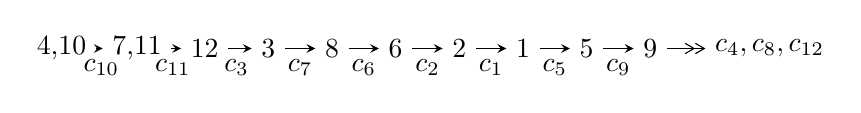
\begin{tikzpicture}[x=23pt, y=7pt]
	% node
	\node (A0) at (-1/8, 0) {4,10};
	\node (A1) at (17/16, 0) {7,11};
	\node (A2) at (17/8, 0) {12};
	\node (A3) at (25/8, 0) {3};
	\node (A4) at (33/8, 0) {8};
	\node (A5) at (41/8, 0) {6};
	\node (A6) at (49/8, 0) {2};
	\node (A7) at (57/8, 0) {1};
	\node (A8) at (65/8, 0) {5};
	\node (A9) at (73/8, 0) {9};
	\node (C1) at (1/2, -1) {$c_{10}$};
	\node (C2) at (13/8, -1) {$c_{11}$};
	\node (C3) at (21/8, -1) {$c_{3}$};
	\node (C4) at (29/8, -1) {$c_{7}$};
	\node (C5) at (37/8, -1) {$c_{6}$};
	\node (C6) at (45/8, -1) {$c_{2}$};
	\node (C7) at (53/8, -1) {$c_{1}$};
	\node (C8) at (61/8, -1) {$c_{5}$};
	\node (C9) at (69/8, -1) {$c_{9}$};
	\node (A10) at (11, 0) {$c_{4},c_{8},c_{12}$};

	% edge
	\draw[->,>=stealth]	
	(A0) edge (A1) (A1) edge (A2) (A2) edge (A3) (A3) edge (A4) (A4) edge (A5) (A5) edge (A6) (A6) edge (A7) (A7) edge (A8) (A8) edge (A9) ;
	\draw[->>,>={angle 60}]	
	(A9) edge (A10);
\end{tikzpicture} \\ 

\end{tabular} \\

\footnotetext{
The image of knot diagram is generated by the software ``\textbf{Draw programme}" developed by Andrew Bartholomew(\url{http://www.layer8.co.uk/maths/draw/index.htm\#Running-draw}), where we modified some parts for our purpose(\url{https://github.com/CATsTAILs/LinksPainter}).
}\phantom \\ \newline 
\centering \textbf{Ideals for irreducible components\footnotemark of $X_{\text{par}}$} 
 
\begin{align*}
I^u_{1}&=\langle 
-5.87440\times10^{71} u^{62}-1.29008\times10^{72} u^{61}+\cdots+1.81459\times10^{71} b-1.38281\times10^{71},\\
\phantom{I^u_{1}}&\phantom{= \langle  }-2.97873\times10^{71} u^{62}+5.61189\times10^{71} u^{61}+\cdots+1.81459\times10^{71} a+2.70646\times10^{72},\;u^{63}+2 u^{62}+\cdots+6 u+1\rangle \\
I^u_{2}&=\langle 
-10479 u^{21}-2016 u^{20}+\cdots+5129 b-19746,\;37379 u^{21}+17665 u^{20}+\cdots+5129 a+15443,\\
\phantom{I^u_{2}}&\phantom{= \langle  }u^{22}+u^{21}+\cdots- u-1\rangle \\
\\
\end{align*}
\raggedright * 2 irreducible components of $\dim_{\mathbb{C}}=0$, with total 85 representations.\\
\footnotetext{All coefficients of polynomials are rational numbers. But the coefficients are sometimes approximated in decimal forms when there is not enough margin.}
\newpage
\renewcommand{\arraystretch}{1}
\centering \section*{I. $I^u_{1}= \langle -5.87\times10^{71} u^{62}-1.29\times10^{72} u^{61}+\cdots+1.81\times10^{71} b-1.38\times10^{71},\;-2.98\times10^{71} u^{62}+5.61\times10^{71} u^{61}+\cdots+1.81\times10^{71} a+2.71\times10^{72},\;u^{63}+2 u^{62}+\cdots+6 u+1 \rangle$}
\flushleft \textbf{(i) Arc colorings}\\
\begin{tabular}{m{7pt} m{180pt} m{7pt} m{180pt} }
\flushright $a_{4}=$&$\begin{pmatrix}0\\u\end{pmatrix}$ \\
\flushright $a_{10}=$&$\begin{pmatrix}1\\0\end{pmatrix}$ \\
\flushright $a_{7}=$&$\begin{pmatrix}1.64155 u^{62}-3.09266 u^{61}+\cdots-78.0276 u-14.9150\\3.23732 u^{62}+7.10951 u^{61}+\cdots+9.94343 u+0.762053\end{pmatrix}$ \\
\flushright $a_{11}=$&$\begin{pmatrix}1\\u^2\end{pmatrix}$ \\
\flushright $a_{12}=$&$\begin{pmatrix}-4.56195 u^{62}-4.68616 u^{61}+\cdots+86.2185 u+15.8520\\-3.41127 u^{62}-5.48261 u^{61}+\cdots+26.0173 u+4.13758\end{pmatrix}$ \\
\flushright $a_{3}=$&$\begin{pmatrix}u\\u^3+u\end{pmatrix}$ \\
\flushright $a_{8}=$&$\begin{pmatrix}3.21507 u^{62}+3.09966 u^{61}+\cdots-48.7262 u-10.7328\\5.23718 u^{62}+12.3432 u^{61}+\cdots+19.3996 u+1.89905\end{pmatrix}$ \\
\flushright $a_{6}=$&$\begin{pmatrix}4.87888 u^{62}+4.01685 u^{61}+\cdots-68.0842 u-14.1530\\3.23732 u^{62}+7.10951 u^{61}+\cdots+9.94343 u+0.762053\end{pmatrix}$ \\
\flushright $a_{2}=$&$\begin{pmatrix}10.1884 u^{62}+21.3682 u^{61}+\cdots-36.8563 u-13.2634\\4.69842 u^{62}+7.98433 u^{61}+\cdots-13.0129 u-2.93288\end{pmatrix}$ \\
\flushright $a_{1}=$&$\begin{pmatrix}9.84597 u^{62}+20.6041 u^{61}+\cdots-38.4795 u-13.7100\\5.22967 u^{62}+9.33504 u^{61}+\cdots-13.8182 u-3.30023\end{pmatrix}$ \\
\flushright $a_{5}=$&$\begin{pmatrix}-5.48003 u^{62}-12.9936 u^{61}+\cdots+17.9312 u+10.1134\\0.614387 u^{62}+2.61208 u^{61}+\cdots-6.75173 u-1.33074\end{pmatrix}$ \\
\flushright $a_{9}=$&$\begin{pmatrix}-6.73921 u^{62}-6.56138 u^{61}+\cdots+85.1609 u+19.5180\\0.137452 u^{62}+2.12280 u^{61}+\cdots+9.76922 u+1.53689\end{pmatrix}$\\&\end{tabular}
\flushleft \textbf{(ii) Obstruction class $= -1$}\\~\\
\flushleft \textbf{(iii) Cusp Shapes $= 3.92172 u^{62}-2.79562 u^{61}+\cdots-66.9143 u-26.6390$}\\~\\
\newpage\renewcommand{\arraystretch}{1}
\flushleft \textbf{(iv) u-Polynomials at the component}\newline \\
\begin{tabular}{m{50pt}|m{274pt}}
Crossings & \hspace{64pt}u-Polynomials at each crossing \\
\hline $$\begin{aligned}c_{1}\end{aligned}$$&$\begin{aligned}
&u^{63}+82 u^{62}+\cdots+19 u+1
\end{aligned}$\\
\hline $$\begin{aligned}c_{2},c_{5}\end{aligned}$$&$\begin{aligned}
&u^{63}+4 u^{62}+\cdots- u+1
\end{aligned}$\\
\hline $$\begin{aligned}c_{3},c_{10}\end{aligned}$$&$\begin{aligned}
&u^{63}+2 u^{62}+\cdots+6 u+1
\end{aligned}$\\
\hline $$\begin{aligned}c_{4}\end{aligned}$$&$\begin{aligned}
&u^{63}-45 u^{61}+\cdots+113780 u+6263
\end{aligned}$\\
\hline $$\begin{aligned}c_{6}\end{aligned}$$&$\begin{aligned}
&u^{63}+6 u^{62}+\cdots+103 u+43
\end{aligned}$\\
\hline $$\begin{aligned}c_{7}\end{aligned}$$&$\begin{aligned}
&u^{63}- u^{62}+\cdots+83083 u+12017
\end{aligned}$\\
\hline $$\begin{aligned}c_{8}\end{aligned}$$&$\begin{aligned}
&u^{63}+11 u^{62}+\cdots+1626730 u+769055
\end{aligned}$\\
\hline $$\begin{aligned}c_{9},c_{12}\end{aligned}$$&$\begin{aligned}
&u^{63}-3 u^{62}+\cdots+4 u+1
\end{aligned}$\\
\hline $$\begin{aligned}c_{11}\end{aligned}$$&$\begin{aligned}
&u^{63}-2 u^{62}+\cdots+197 u+23
\end{aligned}$\\
\hline
\end{tabular}\\~\\
\newpage\renewcommand{\arraystretch}{1}
\flushleft \textbf{(v) Riley Polynomials at the component}\newline \\
\begin{tabular}{m{50pt}|m{274pt}}
Crossings & \hspace{64pt}Riley Polynomials at each crossing \\
\hline $$\begin{aligned}c_{1}\end{aligned}$$&$\begin{aligned}
&y^{63}-190 y^{62}+\cdots-761 y-1
\end{aligned}$\\
\hline $$\begin{aligned}c_{2},c_{5}\end{aligned}$$&$\begin{aligned}
&y^{63}-82 y^{62}+\cdots+19 y-1
\end{aligned}$\\
\hline $$\begin{aligned}c_{3},c_{10}\end{aligned}$$&$\begin{aligned}
&y^{63}+34 y^{62}+\cdots-8 y-1
\end{aligned}$\\
\hline $$\begin{aligned}c_{4}\end{aligned}$$&$\begin{aligned}
&y^{63}-90 y^{62}+\cdots+1565666672 y-39225169
\end{aligned}$\\
\hline $$\begin{aligned}c_{6}\end{aligned}$$&$\begin{aligned}
&y^{63}+10 y^{62}+\cdots+1579 y-1849
\end{aligned}$\\
\hline $$\begin{aligned}c_{7}\end{aligned}$$&$\begin{aligned}
&y^{63}-19 y^{62}+\cdots+1438703057 y-144408289
\end{aligned}$\\
\hline $$\begin{aligned}c_{8}\end{aligned}$$&$\begin{aligned}
&y^{63}-105 y^{62}+\cdots+44795152652180 y-591445593025
\end{aligned}$\\
\hline $$\begin{aligned}c_{9},c_{12}\end{aligned}$$&$\begin{aligned}
&y^{63}+27 y^{62}+\cdots-16 y-1
\end{aligned}$\\
\hline $$\begin{aligned}c_{11}\end{aligned}$$&$\begin{aligned}
&y^{63}+12 y^{62}+\cdots-15287 y-529
\end{aligned}$\\
\hline
\end{tabular}\\~\\
\newpage\flushleft \textbf{(vi) Complex Volumes and Cusp Shapes}
$$\begin{array}{c|c|c}  
\text{Solutions to }I^u_{1}& \I (\text{vol} + \sqrt{-1}CS) & \text{Cusp shape}\\
 \hline 
\begin{aligned}
u &= -0.990747 + 0.105264 I \\
a &= \phantom{-}0.227845 - 0.215922 I \\
b &= \phantom{-}0.595296 + 0.556231 I\end{aligned}
 & -1.43917 - 1.61508 I & -12.00000 + 4.60707 I \\ \hline\begin{aligned}
u &= -0.990747 - 0.105264 I \\
a &= \phantom{-}0.227845 + 0.215922 I \\
b &= \phantom{-}0.595296 - 0.556231 I\end{aligned}
 & -1.43917 + 1.61508 I & -12.00000 - 4.60707 I \\ \hline\begin{aligned}
u &= -0.362778 + 0.887366 I \\
a &= \phantom{-}0.602460 - 0.037525 I \\
b &= \phantom{-}0.740076 - 0.367736 I\end{aligned}
 & \phantom{-}1.42285 + 4.05328 I & -10.60708 - 8.49104 I \\ \hline\begin{aligned}
u &= -0.362778 - 0.887366 I \\
a &= \phantom{-}0.602460 + 0.037525 I \\
b &= \phantom{-}0.740076 + 0.367736 I\end{aligned}
 & \phantom{-}1.42285 - 4.05328 I & -10.60708 + 8.49104 I \\ \hline\begin{aligned}
u &= \phantom{-}0.946133 + 0.149538 I \\
a &= \phantom{-}0.157340 + 0.179031 I \\
b &= -0.703205 + 0.947694 I\end{aligned}
 & -0.51505 + 4.80413 I & -13.8646 - 5.8524 I \\ \hline\begin{aligned}
u &= \phantom{-}0.946133 - 0.149538 I \\
a &= \phantom{-}0.157340 - 0.179031 I \\
b &= -0.703205 - 0.947694 I\end{aligned}
 & -0.51505 - 4.80413 I & -13.8646 + 5.8524 I \\ \hline\begin{aligned}
u &= -0.302806 + 1.009340 I \\
a &= -0.06447 + 2.59329 I \\
b &= \phantom{-}0.79301 - 1.46212 I\end{aligned}
 & \phantom{-}3.40020 + 4.23251 I & \phantom{-0.000000 } 0 \\ \hline\begin{aligned}
u &= -0.302806 - 1.009340 I \\
a &= -0.06447 - 2.59329 I \\
b &= \phantom{-}0.79301 + 1.46212 I\end{aligned}
 & \phantom{-}3.40020 - 4.23251 I & \phantom{-0.000000 } 0 \\ \hline\begin{aligned}
u &= \phantom{-}0.366638 + 1.026710 I \\
a &= \phantom{-}1.75134 - 0.08856 I \\
b &= \phantom{-}0.551334 + 0.324588 I\end{aligned}
 & -7.10790 - 4.96709 I & \phantom{-0.000000 } 0 \\ \hline\begin{aligned}
u &= \phantom{-}0.366638 - 1.026710 I \\
a &= \phantom{-}1.75134 + 0.08856 I \\
b &= \phantom{-}0.551334 - 0.324588 I\end{aligned}
 & -7.10790 + 4.96709 I & \phantom{-0.000000 } 0\\
 \hline 
 \end{array}$$\newpage$$\begin{array}{c|c|c}  
\text{Solutions to }I^u_{1}& \I (\text{vol} + \sqrt{-1}CS) & \text{Cusp shape}\\
 \hline 
\begin{aligned}
u &= \phantom{-}0.432485 + 1.010080 I \\
a &= -0.63914 + 1.30892 I \\
b &= \phantom{-}0.80072 - 1.37567 I\end{aligned}
 & -7.61563 - 1.01111 I & \phantom{-0.000000 } 0 \\ \hline\begin{aligned}
u &= \phantom{-}0.432485 - 1.010080 I \\
a &= -0.63914 - 1.30892 I \\
b &= \phantom{-}0.80072 + 1.37567 I\end{aligned}
 & -7.61563 + 1.01111 I & \phantom{-0.000000 } 0 \\ \hline\begin{aligned}
u &= -1.085820 + 0.228198 I \\
a &= \phantom{-}0.0071519 + 0.0592893 I \\
b &= -0.908974 - 1.015940 I\end{aligned}
 & -9.06594 - 9.39819 I & \phantom{-0.000000 } 0 \\ \hline\begin{aligned}
u &= -1.085820 - 0.228198 I \\
a &= \phantom{-}0.0071519 - 0.0592893 I \\
b &= -0.908974 + 1.015940 I\end{aligned}
 & -9.06594 + 9.39819 I & \phantom{-0.000000 } 0 \\ \hline\begin{aligned}
u &= \phantom{-}0.239732 + 0.837215 I \\
a &= \phantom{-}0.16007 + 1.91347 I \\
b &= -0.875933 - 0.420278 I\end{aligned}
 & -1.11761 - 1.26731 I & -15.1175 + 4.6617 I \\ \hline\begin{aligned}
u &= \phantom{-}0.239732 - 0.837215 I \\
a &= \phantom{-}0.16007 - 1.91347 I \\
b &= -0.875933 + 0.420278 I\end{aligned}
 & -1.11761 + 1.26731 I & -15.1175 - 4.6617 I \\ \hline\begin{aligned}
u &= \phantom{-}0.264496 + 0.829236 I \\
a &= \phantom{-}0.10067 + 1.46934 I \\
b &= -1.175250 - 0.245574 I\end{aligned}
 & -1.14587 - 1.30347 I & -17.5152 + 4.9826 I \\ \hline\begin{aligned}
u &= \phantom{-}0.264496 - 0.829236 I \\
a &= \phantom{-}0.10067 - 1.46934 I \\
b &= -1.175250 + 0.245574 I\end{aligned}
 & -1.14587 + 1.30347 I & -17.5152 - 4.9826 I \\ \hline\begin{aligned}
u &= -0.376805 + 1.065330 I \\
a &= -0.80125 - 1.37166 I \\
b &= -1.200310 + 0.294963 I\end{aligned}
 & -6.60608 + 0.34953 I & \phantom{-0.000000 } 0 \\ \hline\begin{aligned}
u &= -0.376805 - 1.065330 I \\
a &= -0.80125 + 1.37166 I \\
b &= -1.200310 - 0.294963 I\end{aligned}
 & -6.60608 - 0.34953 I & \phantom{-0.000000 } 0\\
 \hline 
 \end{array}$$\newpage$$\begin{array}{c|c|c}  
\text{Solutions to }I^u_{1}& \I (\text{vol} + \sqrt{-1}CS) & \text{Cusp shape}\\
 \hline 
\begin{aligned}
u &= -0.444883 + 1.040440 I \\
a &= \phantom{-}1.288050 + 0.198665 I \\
b &= -1.64815 - 0.93772 I\end{aligned}
 & -7.15825 + 6.18151 I & \phantom{-0.000000 } 0 \\ \hline\begin{aligned}
u &= -0.444883 - 1.040440 I \\
a &= \phantom{-}1.288050 - 0.198665 I \\
b &= -1.64815 + 0.93772 I\end{aligned}
 & -7.15825 - 6.18151 I & \phantom{-0.000000 } 0 \\ \hline\begin{aligned}
u &= \phantom{-}0.266646 + 0.813283 I \\
a &= \phantom{-}0.505244 + 0.982367 I \\
b &= -1.379120 - 0.085398 I\end{aligned}
 & -1.17639 - 1.29143 I & -15.3554 + 5.4557 I \\ \hline\begin{aligned}
u &= \phantom{-}0.266646 - 0.813283 I \\
a &= \phantom{-}0.505244 - 0.982367 I \\
b &= -1.379120 + 0.085398 I\end{aligned}
 & -1.17639 + 1.29143 I & -15.3554 - 5.4557 I \\ \hline\begin{aligned}
u &= -0.896656 + 0.823164 I \\
a &= -0.512264 + 0.204586 I \\
b &= \phantom{-}0.135578 + 0.584282 I\end{aligned}
 & \phantom{-}0.351157 + 0.534295 I & \phantom{-0.000000 } 0 \\ \hline\begin{aligned}
u &= -0.896656 - 0.823164 I \\
a &= -0.512264 - 0.204586 I \\
b &= \phantom{-}0.135578 - 0.584282 I\end{aligned}
 & \phantom{-}0.351157 - 0.534295 I & \phantom{-0.000000 } 0 \\ \hline\begin{aligned}
u &= -0.401918 + 1.182270 I \\
a &= -0.24327 - 1.63490 I \\
b &= -0.48135 + 1.46123 I\end{aligned}
 & \phantom{-}3.27235 + 3.48208 I & \phantom{-0.000000 } 0 \\ \hline\begin{aligned}
u &= -0.401918 - 1.182270 I \\
a &= -0.24327 + 1.63490 I \\
b &= -0.48135 - 1.46123 I\end{aligned}
 & \phantom{-}3.27235 - 3.48208 I & \phantom{-0.000000 } 0 \\ \hline\begin{aligned}
u &= \phantom{-}0.394861 + 1.192190 I \\
a &= \phantom{-}0.12689 - 1.95895 I \\
b &= \phantom{-}0.784716 + 1.058410 I\end{aligned}
 & \phantom{-}6.38319 - 6.23226 I & \phantom{-0.000000 } 0 \\ \hline\begin{aligned}
u &= \phantom{-}0.394861 - 1.192190 I \\
a &= \phantom{-}0.12689 + 1.95895 I \\
b &= \phantom{-}0.784716 - 1.058410 I\end{aligned}
 & \phantom{-}6.38319 + 6.23226 I & \phantom{-0.000000 } 0\\
 \hline 
 \end{array}$$\newpage$$\begin{array}{c|c|c}  
\text{Solutions to }I^u_{1}& \I (\text{vol} + \sqrt{-1}CS) & \text{Cusp shape}\\
 \hline 
\begin{aligned}
u &= -0.154944 + 0.706018 I \\
a &= -0.650670 - 0.500412 I \\
b &= \phantom{-}1.19705 + 0.87628 I\end{aligned}
 & \phantom{-}2.19848 - 1.89748 I & -9.51830 - 4.60789 I \\ \hline\begin{aligned}
u &= -0.154944 - 0.706018 I \\
a &= -0.650670 + 0.500412 I \\
b &= \phantom{-}1.19705 - 0.87628 I\end{aligned}
 & \phantom{-}2.19848 + 1.89748 I & -9.51830 + 4.60789 I \\ \hline\begin{aligned}
u &= -0.367705 + 1.239600 I \\
a &= -0.285293 - 1.181370 I \\
b &= -0.007485 + 0.931592 I\end{aligned}
 & \phantom{-}3.24616 + 2.75157 I & \phantom{-0.000000 } 0 \\ \hline\begin{aligned}
u &= -0.367705 - 1.239600 I \\
a &= -0.285293 + 1.181370 I \\
b &= -0.007485 - 0.931592 I\end{aligned}
 & \phantom{-}3.24616 - 2.75157 I & \phantom{-0.000000 } 0 \\ \hline\begin{aligned}
u &= \phantom{-}0.313182 + 1.259970 I \\
a &= \phantom{-}0.543704 - 0.954155 I \\
b &= \phantom{-}0.172815 + 1.016880 I\end{aligned}
 & \phantom{-}4.29462 + 0.53295 I & \phantom{-0.000000 } 0 \\ \hline\begin{aligned}
u &= \phantom{-}0.313182 - 1.259970 I \\
a &= \phantom{-}0.543704 + 0.954155 I \\
b &= \phantom{-}0.172815 - 1.016880 I\end{aligned}
 & \phantom{-}4.29462 - 0.53295 I & \phantom{-0.000000 } 0 \\ \hline\begin{aligned}
u &= -0.558772 + 1.190380 I \\
a &= \phantom{-}0.410167 + 0.900060 I \\
b &= \phantom{-}0.693773 - 0.904421 I\end{aligned}
 & \phantom{-}2.19335 + 4.97234 I & \phantom{-0.000000 } 0 \\ \hline\begin{aligned}
u &= -0.558772 - 1.190380 I \\
a &= \phantom{-}0.410167 - 0.900060 I \\
b &= \phantom{-}0.693773 + 0.904421 I\end{aligned}
 & \phantom{-}2.19335 - 4.97234 I & \phantom{-0.000000 } 0 \\ \hline\begin{aligned}
u &= \phantom{-}0.604819 + 1.173120 I \\
a &= -0.686547 + 0.580713 I \\
b &= \phantom{-}0.107053 - 0.612042 I\end{aligned}
 & \phantom{-}5.07461 - 2.21684 I & \phantom{-0.000000 } 0 \\ \hline\begin{aligned}
u &= \phantom{-}0.604819 - 1.173120 I \\
a &= -0.686547 - 0.580713 I \\
b &= \phantom{-}0.107053 + 0.612042 I\end{aligned}
 & \phantom{-}5.07461 + 2.21684 I & \phantom{-0.000000 } 0\\
 \hline 
 \end{array}$$\newpage$$\begin{array}{c|c|c}  
\text{Solutions to }I^u_{1}& \I (\text{vol} + \sqrt{-1}CS) & \text{Cusp shape}\\
 \hline 
\begin{aligned}
u &= \phantom{-}0.536211 + 1.239640 I \\
a &= -0.26898 + 1.68491 I \\
b &= -0.95890 - 1.43950 I\end{aligned}
 & \phantom{-}2.83710 - 10.11180 I & \phantom{-0.000000 } 0 \\ \hline\begin{aligned}
u &= \phantom{-}0.536211 - 1.239640 I \\
a &= -0.26898 - 1.68491 I \\
b &= -0.95890 + 1.43950 I\end{aligned}
 & \phantom{-}2.83710 + 10.11180 I & \phantom{-0.000000 } 0 \\ \hline\begin{aligned}
u &= -0.515239 + 1.259240 I \\
a &= \phantom{-}0.30480 + 1.49648 I \\
b &= \phantom{-}0.806111 - 0.864148 I\end{aligned}
 & \phantom{-}2.16604 + 6.91375 I & \phantom{-0.000000 } 0 \\ \hline\begin{aligned}
u &= -0.515239 - 1.259240 I \\
a &= \phantom{-}0.30480 - 1.49648 I \\
b &= \phantom{-}0.806111 + 0.864148 I\end{aligned}
 & \phantom{-}2.16604 - 6.91375 I & \phantom{-0.000000 } 0 \\ \hline\begin{aligned}
u &= \phantom{-}0.608595 + 0.144028 I \\
a &= \phantom{-}0.067285 - 0.477371 I \\
b &= \phantom{-}0.757994 + 0.677519 I\end{aligned}
 & \phantom{-}2.72700 - 2.52576 I & -6.98143 + 1.65333 I \\ \hline\begin{aligned}
u &= \phantom{-}0.608595 - 0.144028 I \\
a &= \phantom{-}0.067285 + 0.477371 I \\
b &= \phantom{-}0.757994 - 0.677519 I\end{aligned}
 & \phantom{-}2.72700 + 2.52576 I & -6.98143 - 1.65333 I \\ \hline\begin{aligned}
u &= \phantom{-}0.054830 + 0.620583 I \\
a &= -0.55470 - 4.38288 I \\
b &= -0.332756 - 0.253543 I\end{aligned}
 & -8.90568 + 2.29149 I & -19.8574 - 3.6503 I \\ \hline\begin{aligned}
u &= \phantom{-}0.054830 - 0.620583 I \\
a &= -0.55470 + 4.38288 I \\
b &= -0.332756 + 0.253543 I\end{aligned}
 & -8.90568 - 2.29149 I & -19.8574 + 3.6503 I \\ \hline\begin{aligned}
u &= -0.606194 + 0.122041 I \\
a &= \phantom{-}0.612063 + 0.621270 I \\
b &= -0.262217 + 0.621399 I\end{aligned}
 & -0.290214 - 0.243550 I & -13.68198 + 0.43894 I \\ \hline\begin{aligned}
u &= -0.606194 - 0.122041 I \\
a &= \phantom{-}0.612063 - 0.621270 I \\
b &= -0.262217 - 0.621399 I\end{aligned}
 & -0.290214 + 0.243550 I & -13.68198 - 0.43894 I\\
 \hline 
 \end{array}$$\newpage$$\begin{array}{c|c|c}  
\text{Solutions to }I^u_{1}& \I (\text{vol} + \sqrt{-1}CS) & \text{Cusp shape}\\
 \hline 
\begin{aligned}
u &= -0.614828 + 1.271960 I \\
a &= -0.31937 - 1.70637 I \\
b &= -1.08251 + 1.27663 I\end{aligned}
 & -5.7998 + 15.4283 I & \phantom{-0.000000 } 0 \\ \hline\begin{aligned}
u &= -0.614828 - 1.271960 I \\
a &= -0.31937 + 1.70637 I \\
b &= -1.08251 - 1.27663 I\end{aligned}
 & -5.7998 - 15.4283 I & \phantom{-0.000000 } 0 \\ \hline\begin{aligned}
u &= \phantom{-}1.40889 + 0.36230 I \\
a &= -0.0311359 + 0.0161896 I \\
b &= \phantom{-}0.478420 - 0.426890 I\end{aligned}
 & -12.34440 + 0.36923 I & \phantom{-0.000000 } 0 \\ \hline\begin{aligned}
u &= \phantom{-}1.40889 - 0.36230 I \\
a &= -0.0311359 - 0.0161896 I \\
b &= \phantom{-}0.478420 + 0.426890 I\end{aligned}
 & -12.34440 - 0.36923 I & \phantom{-0.000000 } 0 \\ \hline\begin{aligned}
u &= \phantom{-}0.69263 + 1.31248 I \\
a &= \phantom{-}0.097753 - 1.087490 I \\
b &= \phantom{-}0.882208 + 0.799377 I\end{aligned}
 & -9.07833 - 7.42766 I & \phantom{-0.000000 } 0 \\ \hline\begin{aligned}
u &= \phantom{-}0.69263 - 1.31248 I \\
a &= \phantom{-}0.097753 + 1.087490 I \\
b &= \phantom{-}0.882208 - 0.799377 I\end{aligned}
 & -9.07833 + 7.42766 I & \phantom{-0.000000 } 0 \\ \hline\begin{aligned}
u &= -0.20493 + 1.49295 I \\
a &= \phantom{-}0.516419 + 0.852002 I \\
b &= -0.329934 - 1.026900 I\end{aligned}
 & -3.00927 - 4.46302 I & \phantom{-0.000000 } 0 \\ \hline\begin{aligned}
u &= -0.20493 - 1.49295 I \\
a &= \phantom{-}0.516419 - 0.852002 I \\
b &= -0.329934 + 1.026900 I\end{aligned}
 & -3.00927 + 4.46302 I & \phantom{-0.000000 } 0 \\ \hline\begin{aligned}
u &= \phantom{-}0.257688 + 0.407987 I \\
a &= \phantom{-}1.88508 - 3.61639 I \\
b &= -0.199922 + 1.300740 I\end{aligned}
 & -9.34370 - 2.46865 I & -15.4465 + 3.3962 I \\ \hline\begin{aligned}
u &= \phantom{-}0.257688 - 0.407987 I \\
a &= \phantom{-}1.88508 + 3.61639 I \\
b &= -0.199922 - 1.300740 I\end{aligned}
 & -9.34370 + 2.46865 I & -15.4465 - 3.3962 I\\
 \hline 
 \end{array}$$\newpage$$\begin{array}{c|c|c}  
\text{Solutions to }I^u_{1}& \I (\text{vol} + \sqrt{-1}CS) & \text{Cusp shape}\\
 \hline 
\begin{aligned}
u &= -0.322413 + 0.231256 I \\
a &= -2.69396 - 3.36716 I \\
b &= -0.793788 + 1.024690 I\end{aligned}
 & -9.22509 - 2.54978 I & -16.0238 + 1.2523 I \\ \hline\begin{aligned}
u &= -0.322413 - 0.231256 I \\
a &= -2.69396 + 3.36716 I \\
b &= -0.793788 - 1.024690 I\end{aligned}
 & -9.22509 + 2.54978 I & -16.0238 - 1.2523 I \\ \hline\begin{aligned}
u &= -0.360773\phantom{ +0.000000I} \\
a &= \phantom{-}0.773414\phantom{ +0.000000I} \\
b &= -0.312684\phantom{ +0.000000I}\end{aligned}
 & -0.615548\phantom{ +0.000000I} & -16.1410\phantom{ +0.000000I}\\
 \hline 
 \end{array}$$\newpage\newpage\renewcommand{\arraystretch}{1}
\centering \section*{II. $I^u_{2}= \langle -10479 u^{21}-2016 u^{20}+\cdots+5129 b-19746,\;37379 u^{21}+17665 u^{20}+\cdots+5129 a+15443,\;u^{22}+u^{21}+\cdots- u-1 \rangle$}
\flushleft \textbf{(i) Arc colorings}\\
\begin{tabular}{m{7pt} m{180pt} m{7pt} m{180pt} }
\flushright $a_{4}=$&$\begin{pmatrix}0\\u\end{pmatrix}$ \\
\flushright $a_{10}=$&$\begin{pmatrix}1\\0\end{pmatrix}$ \\
\flushright $a_{7}=$&$\begin{pmatrix}-7.28778 u^{21}-3.44414 u^{20}+\cdots+10.7421 u-3.01092\\2.04309 u^{21}+0.393059 u^{20}+\cdots-3.29674 u+3.84987\end{pmatrix}$ \\
\flushright $a_{11}=$&$\begin{pmatrix}1\\u^2\end{pmatrix}$ \\
\flushright $a_{12}=$&$\begin{pmatrix}-9.38760 u^{21}-13.6036 u^{20}+\cdots+23.3843 u+11.7306\\3.05108 u^{21}+2.68317 u^{20}+\cdots-7.03958 u+0.405732\end{pmatrix}$ \\
\flushright $a_{3}=$&$\begin{pmatrix}u\\u^3+u\end{pmatrix}$ \\
\flushright $a_{8}=$&$\begin{pmatrix}-4.17235 u^{21}-2.57224 u^{20}+\cdots+7.18698 u-0.399493\\3.95438 u^{21}+1.46617 u^{20}+\cdots-5.97992 u+4.21778\end{pmatrix}$ \\
\flushright $a_{6}=$&$\begin{pmatrix}-5.24469 u^{21}-3.05108 u^{20}+\cdots+7.44531 u+0.838955\\2.04309 u^{21}+0.393059 u^{20}+\cdots-3.29674 u+3.84987\end{pmatrix}$ \\
\flushright $a_{2}=$&$\begin{pmatrix}-5.16650 u^{21}-1.55508 u^{20}+\cdots+6.59466 u-5.01716\\1.12127 u^{21}-0.110938 u^{20}+\cdots+0.852603 u-0.00623903\end{pmatrix}$ \\
\flushright $a_{1}=$&$\begin{pmatrix}-7.12673 u^{21}-2.03841 u^{20}+\cdots+8.16689 u-6.61727\\0.0163775 u^{21}-0.551959 u^{20}+\cdots+1.94151 u-0.129460\end{pmatrix}$ \\
\flushright $a_{5}=$&$\begin{pmatrix}4.62800 u^{21}+0.108793 u^{20}+\cdots-3.52856 u+6.08345\\-0.955937 u^{21}+0.0625853 u^{20}+\cdots+0.271203 u-1.25307\end{pmatrix}$ \\
\flushright $a_{9}=$&$\begin{pmatrix}6.06200 u^{21}+2.98187 u^{20}+\cdots-5.07857 u+0.652759\\-2.21213 u^{21}-2.08891 u^{20}+\cdots+4.61474 u+2.20062\end{pmatrix}$\\&\end{tabular}
\flushleft \textbf{(ii) Obstruction class $= 1$}\\~\\
\flushleft \textbf{(iii) Cusp Shapes $= \frac{27167}{5129} u^{21}+\frac{37974}{5129} u^{20}+\cdots-\frac{138057}{5129} u-\frac{95072}{5129}$}\\~\\
\newpage\renewcommand{\arraystretch}{1}
\flushleft \textbf{(iv) u-Polynomials at the component}\newline \\
\begin{tabular}{m{50pt}|m{274pt}}
Crossings & \hspace{64pt}u-Polynomials at each crossing \\
\hline $$\begin{aligned}c_{1}\end{aligned}$$&$\begin{aligned}
&u^{22}-25 u^{21}+\cdots-94 u+9
\end{aligned}$\\
\hline $$\begin{aligned}c_{2}\end{aligned}$$&$\begin{aligned}
&u^{22}+3 u^{21}+\cdots+4 u-3
\end{aligned}$\\
\hline $$\begin{aligned}c_{3}\end{aligned}$$&$\begin{aligned}
&u^{22}- u^{21}+\cdots+u-1
\end{aligned}$\\
\hline $$\begin{aligned}c_{4}\end{aligned}$$&$\begin{aligned}
&u^{22}+3 u^{21}+\cdots+9 u-1
\end{aligned}$\\
\hline $$\begin{aligned}c_{5}\end{aligned}$$&$\begin{aligned}
&u^{22}-3 u^{21}+\cdots-4 u-3
\end{aligned}$\\
\hline $$\begin{aligned}c_{6}\end{aligned}$$&$\begin{aligned}
&u^{22}+u^{21}+\cdots-6 u+1
\end{aligned}$\\
\hline $$\begin{aligned}c_{7}\end{aligned}$$&$\begin{aligned}
&u^{22}-3 u^{20}+\cdots-42 u-7
\end{aligned}$\\
\hline $$\begin{aligned}c_{8}\end{aligned}$$&$\begin{aligned}
&u^{22}+16 u^{21}+\cdots-21 u+1
\end{aligned}$\\
\hline $$\begin{aligned}c_{9}\end{aligned}$$&$\begin{aligned}
&u^{22}-2 u^{21}+\cdots-7 u+7
\end{aligned}$\\
\hline $$\begin{aligned}c_{10}\end{aligned}$$&$\begin{aligned}
&u^{22}+u^{21}+\cdots- u-1
\end{aligned}$\\
\hline $$\begin{aligned}c_{11}\end{aligned}$$&$\begin{aligned}
&u^{22}+u^{21}+\cdots+10 u-3
\end{aligned}$\\
\hline $$\begin{aligned}c_{12}\end{aligned}$$&$\begin{aligned}
&u^{22}+2 u^{21}+\cdots+7 u+7
\end{aligned}$\\
\hline
\end{tabular}\\~\\
\newpage\renewcommand{\arraystretch}{1}
\flushleft \textbf{(v) Riley Polynomials at the component}\newline \\
\begin{tabular}{m{50pt}|m{274pt}}
Crossings & \hspace{64pt}Riley Polynomials at each crossing \\
\hline $$\begin{aligned}c_{1}\end{aligned}$$&$\begin{aligned}
&y^{22}-45 y^{21}+\cdots-970 y+81
\end{aligned}$\\
\hline $$\begin{aligned}c_{2},c_{5}\end{aligned}$$&$\begin{aligned}
&y^{22}-25 y^{21}+\cdots-94 y+9
\end{aligned}$\\
\hline $$\begin{aligned}c_{3},c_{10}\end{aligned}$$&$\begin{aligned}
&y^{22}+11 y^{21}+\cdots+5 y+1
\end{aligned}$\\
\hline $$\begin{aligned}c_{4}\end{aligned}$$&$\begin{aligned}
&y^{22}-17 y^{21}+\cdots+y+1
\end{aligned}$\\
\hline $$\begin{aligned}c_{6}\end{aligned}$$&$\begin{aligned}
&y^{22}+3 y^{21}+\cdots-18 y+1
\end{aligned}$\\
\hline $$\begin{aligned}c_{7}\end{aligned}$$&$\begin{aligned}
&y^{22}-6 y^{21}+\cdots-504 y+49
\end{aligned}$\\
\hline $$\begin{aligned}c_{8}\end{aligned}$$&$\begin{aligned}
&y^{22}-20 y^{21}+\cdots-315 y+1
\end{aligned}$\\
\hline $$\begin{aligned}c_{9},c_{12}\end{aligned}$$&$\begin{aligned}
&y^{22}+16 y^{21}+\cdots+525 y+49
\end{aligned}$\\
\hline $$\begin{aligned}c_{11}\end{aligned}$$&$\begin{aligned}
&y^{22}+9 y^{21}+\cdots-52 y+9
\end{aligned}$\\
\hline
\end{tabular}\\~\\
\newpage\flushleft \textbf{(vi) Complex Volumes and Cusp Shapes}
$$\begin{array}{c|c|c}  
\text{Solutions to }I^u_{2}& \I (\text{vol} + \sqrt{-1}CS) & \text{Cusp shape}\\
 \hline 
\begin{aligned}
u &= \phantom{-}0.215981 + 0.880776 I \\
a &= \phantom{-}0.42291 + 1.74778 I \\
b &= -1.40489 - 0.32594 I\end{aligned}
 & -0.729664 - 1.055600 I & -2.65388 - 3.37536 I \\ \hline\begin{aligned}
u &= \phantom{-}0.215981 - 0.880776 I \\
a &= \phantom{-}0.42291 - 1.74778 I \\
b &= -1.40489 + 0.32594 I\end{aligned}
 & -0.729664 + 1.055600 I & -2.65388 + 3.37536 I \\ \hline\begin{aligned}
u &= -0.311175 + 1.080890 I \\
a &= -0.488004 + 0.062463 I \\
b &= -0.745155 - 0.531362 I\end{aligned}
 & -6.87085 + 3.84054 I & -10.78288 - 1.99979 I \\ \hline\begin{aligned}
u &= -0.311175 - 1.080890 I \\
a &= -0.488004 - 0.062463 I \\
b &= -0.745155 + 0.531362 I\end{aligned}
 & -6.87085 - 3.84054 I & -10.78288 + 1.99979 I \\ \hline\begin{aligned}
u &= \phantom{-}1.031220 + 0.501169 I \\
a &= -0.131657 + 0.134690 I \\
b &= \phantom{-}0.195174 + 0.546308 I\end{aligned}
 & \phantom{-}0.292897 - 1.232480 I & -9.81223 + 6.77489 I \\ \hline\begin{aligned}
u &= \phantom{-}1.031220 - 0.501169 I \\
a &= -0.131657 - 0.134690 I \\
b &= \phantom{-}0.195174 - 0.546308 I\end{aligned}
 & \phantom{-}0.292897 + 1.232480 I & -9.81223 - 6.77489 I \\ \hline\begin{aligned}
u &= -0.110176 + 0.792347 I \\
a &= \phantom{-}0.50663 - 4.05553 I \\
b &= -0.336422 + 0.901790 I\end{aligned}
 & -8.34331 - 2.04079 I & -6.73669 - 1.53590 I \\ \hline\begin{aligned}
u &= -0.110176 - 0.792347 I \\
a &= \phantom{-}0.50663 + 4.05553 I \\
b &= -0.336422 - 0.901790 I\end{aligned}
 & -8.34331 + 2.04079 I & -6.73669 + 1.53590 I \\ \hline\begin{aligned}
u &= \phantom{-}0.342652 + 1.196430 I \\
a &= \phantom{-}0.00858 - 1.86730 I \\
b &= \phantom{-}0.43597 + 1.36736 I\end{aligned}
 & \phantom{-}5.26394 - 4.40995 I & -6.55309 + 3.89134 I \\ \hline\begin{aligned}
u &= \phantom{-}0.342652 - 1.196430 I \\
a &= \phantom{-}0.00858 + 1.86730 I \\
b &= \phantom{-}0.43597 - 1.36736 I\end{aligned}
 & \phantom{-}5.26394 + 4.40995 I & -6.55309 - 3.89134 I\\
 \hline 
 \end{array}$$\newpage$$\begin{array}{c|c|c}  
\text{Solutions to }I^u_{2}& \I (\text{vol} + \sqrt{-1}CS) & \text{Cusp shape}\\
 \hline 
\begin{aligned}
u &= -0.476115 + 1.200480 I \\
a &= \phantom{-}0.33709 + 1.86499 I \\
b &= \phantom{-}1.06414 - 1.14093 I\end{aligned}
 & \phantom{-}5.11201 + 7.58757 I & -9.27554 - 6.67902 I \\ \hline\begin{aligned}
u &= -0.476115 - 1.200480 I \\
a &= \phantom{-}0.33709 - 1.86499 I \\
b &= \phantom{-}1.06414 + 1.14093 I\end{aligned}
 & \phantom{-}5.11201 - 7.58757 I & -9.27554 + 6.67902 I \\ \hline\begin{aligned}
u &= -0.682738 + 0.059063 I \\
a &= \phantom{-}0.528403 + 0.030745 I \\
b &= \phantom{-}0.879737 + 0.878115 I\end{aligned}
 & \phantom{-}1.84449 - 3.13922 I & -13.7549 + 4.3871 I \\ \hline\begin{aligned}
u &= -0.682738 - 0.059063 I \\
a &= \phantom{-}0.528403 - 0.030745 I \\
b &= \phantom{-}0.879737 - 0.878115 I\end{aligned}
 & \phantom{-}1.84449 + 3.13922 I & -13.7549 - 4.3871 I \\ \hline\begin{aligned}
u &= -0.492309 + 1.236030 I \\
a &= -0.723571 - 0.734040 I \\
b &= \phantom{-}0.310470 + 1.012790 I\end{aligned}
 & \phantom{-}5.07188 + 1.32197 I & -7.08101 + 1.81161 I \\ \hline\begin{aligned}
u &= -0.492309 - 1.236030 I \\
a &= -0.723571 + 0.734040 I \\
b &= \phantom{-}0.310470 - 1.012790 I\end{aligned}
 & \phantom{-}5.07188 - 1.32197 I & -7.08101 - 1.81161 I \\ \hline\begin{aligned}
u &= -0.113901 + 0.608983 I \\
a &= \phantom{-}0.16460 + 1.46569 I \\
b &= \phantom{-}1.005810 - 0.896390 I\end{aligned}
 & \phantom{-}2.12223 + 2.58152 I & -10.96980 - 5.73632 I \\ \hline\begin{aligned}
u &= -0.113901 - 0.608983 I \\
a &= \phantom{-}0.16460 - 1.46569 I \\
b &= \phantom{-}1.005810 + 0.896390 I\end{aligned}
 & \phantom{-}2.12223 - 2.58152 I & -10.96980 + 5.73632 I \\ \hline\begin{aligned}
u &= \phantom{-}0.569626 + 1.287640 I \\
a &= -0.492631 + 0.851572 I \\
b &= -0.436703 - 0.769932 I\end{aligned}
 & \phantom{-}3.33386 - 4.94613 I & -6.20084 + 4.11530 I \\ \hline\begin{aligned}
u &= \phantom{-}0.569626 - 1.287640 I \\
a &= -0.492631 - 0.851572 I \\
b &= -0.436703 + 0.769932 I\end{aligned}
 & \phantom{-}3.33386 + 4.94613 I & -6.20084 - 4.11530 I\\
 \hline 
 \end{array}$$\newpage$$\begin{array}{c|c|c}  
\text{Solutions to }I^u_{2}& \I (\text{vol} + \sqrt{-1}CS) & \text{Cusp shape}\\
 \hline 
\begin{aligned}
u &= -1.43376\phantom{ +0.000000I} \\
a &= -0.278601\phantom{ +0.000000I} \\
b &= -0.203139\phantom{ +0.000000I}\end{aligned}
 & -12.0426\phantom{ +0.000000I} & -4.69420\phantom{ +0.000000I} \\ \hline\begin{aligned}
u &= \phantom{-}0.487622\phantom{ +0.000000I} \\
a &= -0.986099\phantom{ +0.000000I} \\
b &= -0.733122\phantom{ +0.000000I}\end{aligned}
 & -2.15240\phantom{ +0.000000I} & -18.6640\phantom{ +0.000000I}\\
 \hline 
 \end{array}$$\newpage
\newpage\renewcommand{\arraystretch}{1}
\centering \section*{ III. u-Polynomials}
\begin{tabular}{m{50pt}|m{274pt}}
Crossings & \hspace{64pt}u-Polynomials at each crossing \\
\hline $$\begin{aligned}c_{1}\end{aligned}$$&$\begin{aligned}
&(u^{22}-25 u^{21}+\cdots-94 u+9)(u^{63}+82 u^{62}+\cdots+19 u+1)
\end{aligned}$\\
\hline $$\begin{aligned}c_{2}\end{aligned}$$&$\begin{aligned}
&(u^{22}+3 u^{21}+\cdots+4 u-3)(u^{63}+4 u^{62}+\cdots- u+1)
\end{aligned}$\\
\hline $$\begin{aligned}c_{3}\end{aligned}$$&$\begin{aligned}
&(u^{22}- u^{21}+\cdots+u-1)(u^{63}+2 u^{62}+\cdots+6 u+1)
\end{aligned}$\\
\hline $$\begin{aligned}c_{4}\end{aligned}$$&$\begin{aligned}
&(u^{22}+3 u^{21}+\cdots+9 u-1)(u^{63}-45 u^{61}+\cdots+113780 u+6263)
\end{aligned}$\\
\hline $$\begin{aligned}c_{5}\end{aligned}$$&$\begin{aligned}
&(u^{22}-3 u^{21}+\cdots-4 u-3)(u^{63}+4 u^{62}+\cdots- u+1)
\end{aligned}$\\
\hline $$\begin{aligned}c_{6}\end{aligned}$$&$\begin{aligned}
&(u^{22}+u^{21}+\cdots-6 u+1)(u^{63}+6 u^{62}+\cdots+103 u+43)
\end{aligned}$\\
\hline $$\begin{aligned}c_{7}\end{aligned}$$&$\begin{aligned}
&(u^{22}-3 u^{20}+\cdots-42 u-7)(u^{63}- u^{62}+\cdots+83083 u+12017)
\end{aligned}$\\
\hline $$\begin{aligned}c_{8}\end{aligned}$$&$\begin{aligned}
&(u^{22}+16 u^{21}+\cdots-21 u+1)\\
&\cdot(u^{63}+11 u^{62}+\cdots+1626730 u+769055)
\end{aligned}$\\
\hline $$\begin{aligned}c_{9}\end{aligned}$$&$\begin{aligned}
&(u^{22}-2 u^{21}+\cdots-7 u+7)(u^{63}-3 u^{62}+\cdots+4 u+1)
\end{aligned}$\\
\hline $$\begin{aligned}c_{10}\end{aligned}$$&$\begin{aligned}
&(u^{22}+u^{21}+\cdots- u-1)(u^{63}+2 u^{62}+\cdots+6 u+1)
\end{aligned}$\\
\hline $$\begin{aligned}c_{11}\end{aligned}$$&$\begin{aligned}
&(u^{22}+u^{21}+\cdots+10 u-3)(u^{63}-2 u^{62}+\cdots+197 u+23)
\end{aligned}$\\
\hline $$\begin{aligned}c_{12}\end{aligned}$$&$\begin{aligned}
&(u^{22}+2 u^{21}+\cdots+7 u+7)(u^{63}-3 u^{62}+\cdots+4 u+1)
\end{aligned}$\\
\hline
\end{tabular}\newpage\renewcommand{\arraystretch}{1}
\centering \section*{ IV. Riley Polynomials}
\begin{tabular}{m{50pt}|m{274pt}}
Crossings & \hspace{64pt}Riley Polynomials at each crossing \\
\hline $$\begin{aligned}c_{1}\end{aligned}$$&$\begin{aligned}
&(y^{22}-45 y^{21}+\cdots-970 y+81)(y^{63}-190 y^{62}+\cdots-761 y-1)
\end{aligned}$\\
\hline $$\begin{aligned}c_{2},c_{5}\end{aligned}$$&$\begin{aligned}
&(y^{22}-25 y^{21}+\cdots-94 y+9)(y^{63}-82 y^{62}+\cdots+19 y-1)
\end{aligned}$\\
\hline $$\begin{aligned}c_{3},c_{10}\end{aligned}$$&$\begin{aligned}
&(y^{22}+11 y^{21}+\cdots+5 y+1)(y^{63}+34 y^{62}+\cdots-8 y-1)
\end{aligned}$\\
\hline $$\begin{aligned}c_{4}\end{aligned}$$&$\begin{aligned}
&(y^{22}-17 y^{21}+\cdots+y+1)\\
&\cdot(y^{63}-90 y^{62}+\cdots+1565666672 y-39225169)
\end{aligned}$\\
\hline $$\begin{aligned}c_{6}\end{aligned}$$&$\begin{aligned}
&(y^{22}+3 y^{21}+\cdots-18 y+1)(y^{63}+10 y^{62}+\cdots+1579 y-1849)
\end{aligned}$\\
\hline $$\begin{aligned}c_{7}\end{aligned}$$&$\begin{aligned}
&(y^{22}-6 y^{21}+\cdots-504 y+49)\\
&\cdot(y^{63}-19 y^{62}+\cdots+1438703057 y-144408289)
\end{aligned}$\\
\hline $$\begin{aligned}c_{8}\end{aligned}$$&$\begin{aligned}
&(y^{22}-20 y^{21}+\cdots-315 y+1)\\
&\cdot(y^{63}-105 y^{62}+\cdots+44795152652180 y-591445593025)
\end{aligned}$\\
\hline $$\begin{aligned}c_{9},c_{12}\end{aligned}$$&$\begin{aligned}
&(y^{22}+16 y^{21}+\cdots+525 y+49)(y^{63}+27 y^{62}+\cdots-16 y-1)
\end{aligned}$\\
\hline $$\begin{aligned}c_{11}\end{aligned}$$&$\begin{aligned}
&(y^{22}+9 y^{21}+\cdots-52 y+9)(y^{63}+12 y^{62}+\cdots-15287 y-529)
\end{aligned}$\\
\hline
\end{tabular}
\vskip 2pc
\end{document}